\chapter{Virtuelle Private Netzwerke}

Der Zugriff aus der Ferne auf das lokale Firmennetzwerk ist für verschiedene Anwendungsszenarien unabdingbar. Die Vernetzung von Firmenstandorten, der Zugriff von mobilen Mitarbeitern auf das Firmennetz oder auch ein Zugang für Geschäftspartner auf das Intranet des Unternehmens müssen sicher Umgesetzt werden.
Die Technologie, die dies ermöglichen soll ist \emph{VPN}. Ein VPN ist ein virtuelles privates Netz, eine logische Verbindung die auf einem anderen, physischen Netz aufgebaut wird \cite{zisler2018computer}. Grundsätzlich eignet sich jedes Netz, hier wird jedoch nur die Verwirklichung von VPN über das Internet betrachtet. Es wird unter anderem wird zwischen folgenden Varianten unterschieden:
\begin{itemize}
  \item Site-to-Site/ Branch Office VPN: Verbindung von verschiedenen Firmenstandorten,
  \item End-to-Site/ Remote Access VPN: Verbindung eines Heimarbeitsplatzes oder eines Mobilen Mitarbeiters it dem Intranet des Unternehmens.
  \item End-toEnd VPN: Verbindung zweier Endgeräte,
  \item Extranet VPN: gewährt einem Geschäftspartner/Kunden/Lieferanten Zugang zu Teilen des Internen Netzes 
\end{itemize}

Die Umsetzung des VPN kann entweder bei einem Dienstleister eingekauft werden, dies nennt sich \emph{Trusted VPN}, oder selber als \emph{secure VPN} aufgebaut werden. Beim Einsatz von Trusted VPN sollten vertrauliche Daten zusätzlich auf Anwendungsebene verschlüsselt werden, um sie zum Beispiel vor Innentätern des Dienstleisters zu schützen. 
 Es gibt außerdem Zwischenformen, so dass nur Teile der Technologie bei einem Dienstleister eingekauft werden.


\section{Funktionsweise}

Die Basistechnologie die einem VPN zugrunde liegt ist das \emph{Tunneling}. Es handelt sich um ein Verfahren, welches  Netzwerkprotokolle in beliebige andere Netzwerkprotokolle kapselt (\emph{encapsulation}), über ein Netzwerk verschickt und an einem gegebenen Endpunkt wieder auspackt (\emph{decapsulation}). Das Tunneling kann auf verschiedenen Schichten des Protokollstapels (vergl. Anhang \ref{A1}) ansetzten. Das Prinzip des Tunneling ist in Abbildung \ref{tunnel} dargestellt. Während der Übertragung durch das Internet ist für die Weiterleitung der Datenpakete nicht relevant, dass es sich um Pakete eines virtuellen Netzwerks handelt, hier werden nur die Header X und Y ausgewertet. Die Header A und B sind für den Transport außerhalb der Endpunkte des VPNs zu verwenden. Der Header de Tunneling-Protokolls gibt dem Empfänger am Endpunkt des Tunnels Informationen darüber, wie das Paket weiterzuleiten ist. 

\begin{figure}[h]
	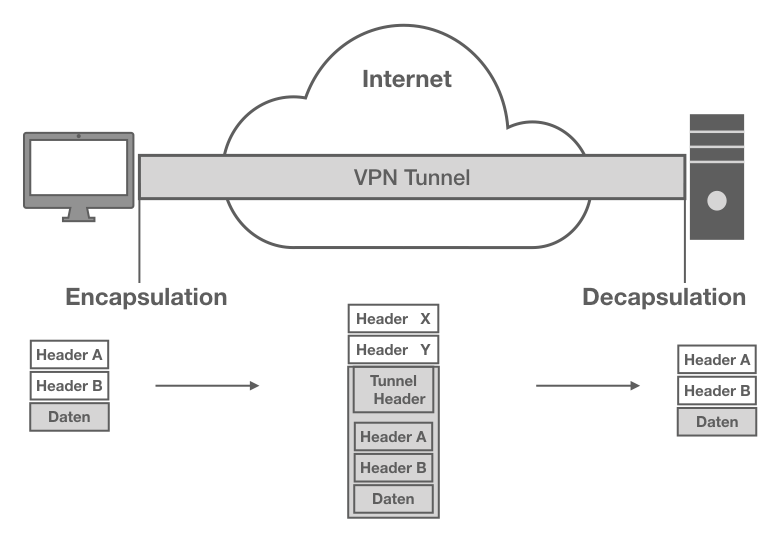
\includegraphics[width=\linewidth]{tunneling}
	\caption{Grundprinzip des Tunneling}
	\label{tunnel}
\end{figure}

 Im Folgenden sollen die wichtigsten standardisierten  Tunneling Protokolle zur VPN-Realisierung vorgestellt werden

\subsection{Layer-2-Protokolle}
Tunneling Protokolle die auf der Sicherungsschicht arbeiten, könne auch in nicht IP-Netzen betrieben werden, da sie unterhalb der IP-Schicht ansetzen. Die verbreitetsten sind das PPTP (Point-to-Poit-Tunneling-Protocol), das L2F  (Layer-two-Forwarding) und das L2TP (Layer two Tunneling Protocol). Da L2TP eine Weiterentwicklung der beiden anderen Protokolle ist \cite{lipp2007vpn} wird dieses stellvertreted für Tunnelingprotokolle auf der Sicherungsschicht im Folgenden näher beschrieben.


\subsubsection{Layer 2 Tunneling Protocol (L2TP)}
Das L2TP ist der Nachfolger der Tunneling Protokolle PPTP und L2F \cite{isi-vpn}. Es kapselt Daten in PPP (Point-to-Point-Protocol \footnote{spezifiziert in RFC 1661: https://www.rfc-editor.org/rfc/rfc1661.txt}) Rahmen, ein Ende-zu-Ende Protokoll auf der Vermittlungsschicht, somit ist es möglich auch nicht-IP Pakete über das Internet zu transportieren \cite{gokulakrishnan2014survey}. Zur Authentisierung dienen die Protokolle EAP (Extensible Authentication Protocol) und CHAP (Challenge Handshake Protocol), die von PPP übernommen werden. Wobei CHAP nach \cite{eckert2018sicherheit} veraltet ist. 
Es können mehrere Verbindungen über einen einzigen L2TP Tunnel laufen, auch alle Management und Wartungsinformationen werden über diesen einen Tunnel ausgetauscht \cite{bohmer2005vpn}.

Da weder L2TP noch PPP die Vertraulichkeit der Daten gewähren, muss die Kommunikation zusätzlich abgesichert werden, dies kann bei Datenverkehr über das Internet mit IPSec (siehe Abschnitt \ref{subsub:L3}) umgesetzt werden. 
Das Haupteinsatzgeiet eines VPNs über L2TP ist ein Site-to-Site oder eines Telearbeitsplatzes.   

\subsection{Layer-3-Protokolle}
Bei Layer-3-Protokolle erfolgt die Kapselung der Daten auf der Vermittlungsschicht, auch Internetschicht oder Netzwerkschicht genannt. Ein Standardprotokoll zur Herstellung von VPN-Verbindungen auf dieser Ebene ist IPSec.

\subsubsection{Internet Protokol Security (IPSec)}
\label{subsub:L3}
Internet Protocol Security (IPSec) ist ein Internetprotokoll bestehend aus drei Komponeneten: dem IP Authentication Header (AH) zur Authentisierung, dem Encapsulating Security Payload (ESP) ebenfalls zur Authentisierung und zur Verschlüsselung der Daten und dem Internet Key Exchange (IKEv2) das zum Schlüsselaustausch und dem Verbindungsaufbau dient\footnote{Spezifiziert werden die Protokolle in den RFCs 4301,4302,4303 und 4306.}. Das AH und das ESP können einzeln oder zusammen genutzt werden. Da AH keine Verschlüsselung bietet ist für die Kommunikation über das Internet das ESP vorzuziehen. AH ist zur Authentifikation der Kommunikation in einem sicheren Netz geeignet \cite{isi-vpn}. Implementierungen von IPSec müssen deswegen ESP zur Verfügung stellen, die Einbindung von AH ist optional.

Sowohl für End-to-End, Site-to-Site und End-to-Site Verbindungen kann IPSec genutzt werden \cite{rfc4301}.

 Es gibt vielfältige Möglichkeiten IPSec zu konfigurieren, so ist zu beachten, dass es möglich ist ESP zu nutzen und dabei nur die Vertraulichkeit, nicht aber die Integrität sicherzustellen. Desweiteren besteht die Möglichkeit einen oder mehrere Tunnel für die Kommunikation zu nutzen. Die Sicherheit der Kommunikation  über IPSec ist abhängig von einer gewissenhaften Implementierung, Konfiguration und einer sicheren Systemumgebung \cite{rfc4301}. 
  
  IPSec ist sowohl für IPv4 als auch für IPv6 definiert, in IPv6 ist es bereits integriert.
\\

Es gibt zwei Benutzungsmodi: den Transportmodus und den Tunnelmodus. Im  Tunnelmodus kann ein klassisches VPN betrieben werden, hier werden IP-Pakete in anderen IP-Paketen gekapselt. Es wird also das gesamte IP-Paket geschützt, inklusive der getunnelten IP-Headerinformationen wie die tatsächliche Ziel und Absenderadresse. Ein Sicherheitsgateway, welches IPSec anbietet muss den Tunnelmodus implementieren und sollte auch dieses verwenden, der Transport von Daten im Transportmodus ist für Sicherheitsgateways nur in Ausnahmefällen erlaubt \cite{rfc4301}. 
\begin{figure}[h]
	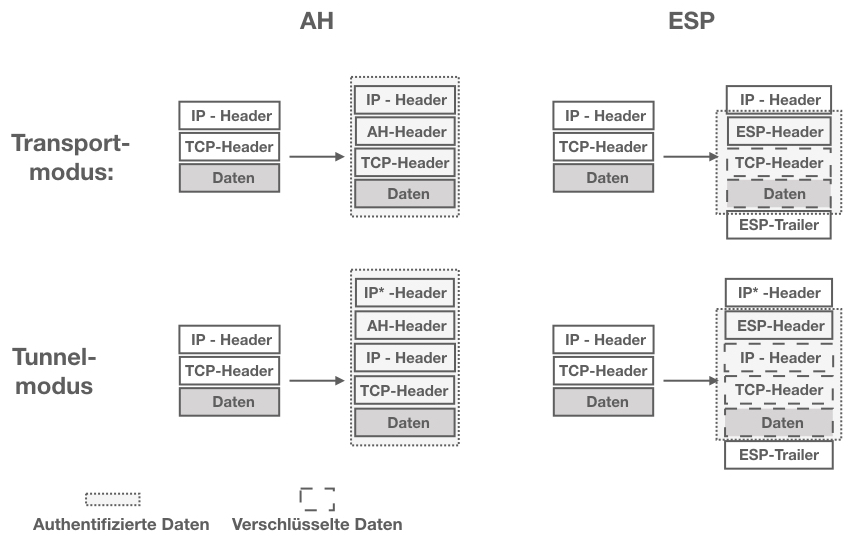
\includegraphics[width=\linewidth]{ahsep.001.jpeg}
	\caption{Transportmodus und Tunnelmodus des IPSec nach \cite{lipp2007vpn}}
	\label{ahesp}
\end{figure}
Im Transportmodus werden die IP-Pakete nicht getunnelt sondern nur ihre Authentizitat und Integrität mittels AH ge\-währleistet oder zusätzlich die Vertraulichkeit mittels ESP. 

Abbildung \ref{ahesp} zeigt den Unterschied von Transport und Tunnelmodes anhand der Paketstruktur unter Benutzung von AH und ESP. Während im Transportmodus der AH- bzw. ESP-Header  hinter dem bestehenden IP-Header eingefügt wird, wird im Tunnelmodus ein neuer IP-Header (hier IP*) erzeugt auf den dann der AH/ESP-Header folgt und anschließend das Original IP-Paket als Nutzlast. Bei ESP folgt sowohl im Transportmodus als auch im Tunnelmodus ein Trailer der die Authentifizierungsdaten enthält. Für ESP ist außerdem zusätzlich angegeben welche Daten verschlüsselt werden, nämlich das gesamte Ursprüngleich  IP-Paket im Fall des Tunnelmoduses oder nur das Paket der Transportschicht, also  das TCP-Paket, im Fall des Transportmodus. 

Die Grafik zeigt außerdem einen weiteren Unterschied zwischen ESP und AH: der Datenbereich der authentifiziert wird unterscheidet sich bei diesen beiden Protokollen. Bei der Benutzung von AH sind Authentizität und Integrität des Pakets inklusive IP-Header, bzw. äußeren IP-Headers im Tunnelmodus,  geschützt, da hier die unveränderlichen Daten des IP-Headers mit einbezogen werden. Dies gestaltet sich allerdings problematisch bei der Verwendung von NAT (Network Address Translation), hier kann AH nicht verwendet werden. 
ESP schützt jeweils den IP-Header nicht mit und kann somit auch bei Verwendung von NAT genutzt werden. 

 
\subsection{Anwendungsschicht VPN}

Der Begriff VPN wird in der Literatur auch für verschlüsselte Verbindungen verwendet. So wird zum Beispiel die Verbindung über SSL bzw. TLS (Secure Socket Layer bzw. Transport Layer Security) als VPN bezeichnet \cite{isi-vpn} \cite{singh2012enhancing}, obwohl hier kein Tunnel aufgebaut wird, sondern verschlüsselte Verbindungen zwischen einzelnen Anwendungen aufgebaut werden. Die Protokolle TLS und SSL sind im Protokollstapel (vgl. Anhang \ref{A1}) zwischen Anwendungsschicht und Transportschicht angesiedelt. 

\section{Sicherheitsmaßnahmen}
Da über die virtuellen Netze sensible Firmendaten über das Internet ausgetauscht werden und evtl. voller Zugriff auf das Firmennetz besteht \cite{singh2012enhancing}, sind VPN Verbindungen besonders abzusichern. Das beginnt bei einer sorgfältigen Planung und Umsetzung des VPN Einsatzes bestehend aus den Teilaufgaben \cite{bsivpn}: 
\begin{itemize}
	\item Anforderungsanalyse
	\item Planung 
	\item Beschaffung
	\item Umsetzung 
	\item Betrieb
	\item Aussonderung (Abschaltung nicht mehr benötigter Zugänge)
	\item Notfallvorsorge.
\end{itemize} 
Zu jedem Aufgabenteil gibt es auf der Webseite des BSI ein oder mehrere Bausteine. 
Dabei sollte als Teil der IT-Sicherheitsleitlinie des Unternehmens auch eine VPN-Sicherheitsleitlinie erstellt werden. 
Auch wenn die Maßnahmenkataloge des BSI sich in erster Linie an Behörden und große Unternehmen richten, sind sie auch für kleine Unternehmen relevant. In vielen Bausteinen werden Varianten für kleine Unternehmen vorgestellt, des Weiteren wird das Erstellen einer Sicherheitsleitlinie auch für kleine Unternehmen empfohlen. 





\subsection{Sichere Netzwerkanbindung}
Das VPN-Gateway kann an verschieden Stellen an das Netzwerk angeschlossen werden. Liegt eine P-A-P Struktur zwischen Internet und Intranet vor empfiehlt das BSI die in Abbildung \ref{vpnarch} gezeigte Anbindung des VPN-Gateways \cite{isi-lana}. 

\begin{figure}[h]
	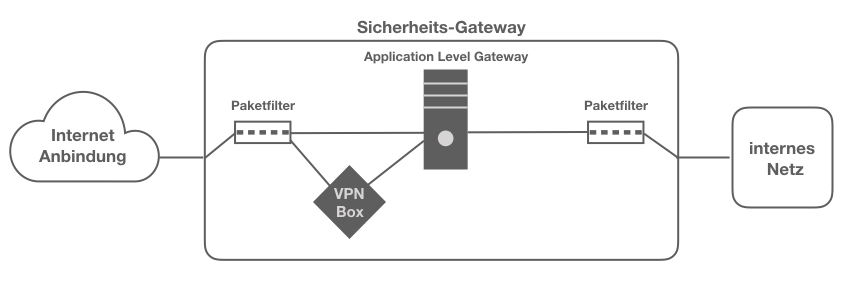
\includegraphics[width=\linewidth]{vpnarchitektur.jpeg}
	\caption{Sichere Einbindung eines VPN-Gateways in eine P-A-P Struktur}
	\label{vpnarch}
\end{figure}

Durch die Platzierung hinter dem zum Internet gerichteten Paketfilter, ist die VPN-Gateway vor Angriffen aus dem Internet geschützt und durch die Platzierung vor dem ALG kann die eingehende Kommunikation entschlüsselt und auch auf Anwendungsebene Untersucht werden \cite{bsivpnaufbau}.\\
 
%Erfolgt die Anbindung an das Internet aus Kostengründen mit nur einer Firewall

\section{VPN in privaten Haushalten}

Virtuelle private Netzwerke werden auch im privaten Bereich  verwendet. Hier gibt es verschiedene Anwendungsszenarien: der Zugriff aus der Ferne auf das Heimnetzwerk zum Beispiel zur Bedienung des IoT (Internet of Things) oder der Zugriff auf die NAS als Cloud-Alternative, als Technologie zum Anonymen surfen im Internet oder zum Überwinden von Geoblocking, oder um seine eigene Sicherheit beim Internetzugang über einen öffentlichen unsicheren Zugangspunkt zu wahren. Auch das BSI empfielht  Privatpersonen ausdrücklich die Nutzung eines VPNs beim surfen in unsicheren WLAN HotSpots \cite{bsibuergervpn}.

In Länder in denen Regierungen stark in die Nutzung des Internets eingreifen und diese einschränken, ist die Nutzung von VPN populär um diese Einschränkungen zu umgehen.\\


\begin{figure}[h]
	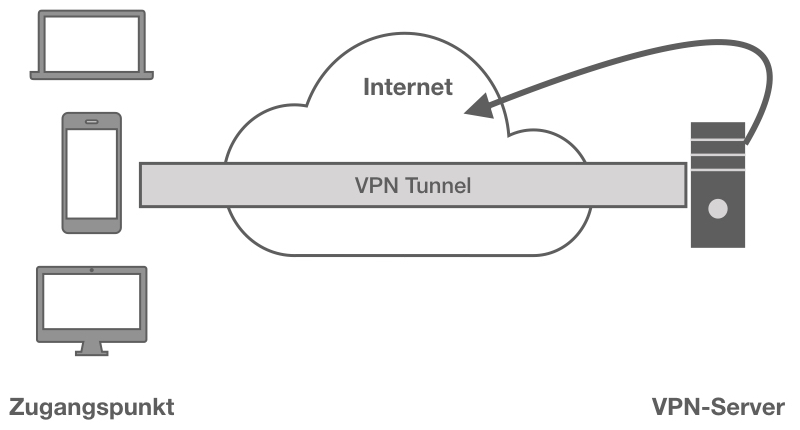
\includegraphics[width=\linewidth,height=8cm]{vpnPrivat.001.jpeg}
	\caption{Schema eines VPNs zur Anonymen Internetnutzung.}
	\label{vpnPrivat}
\end{figure}

VPN wird also nicht ausschließlich genutzt, um aus der Ferne auf ein bestimmtes Intranet, bzw. sein Heimnetz zuzugreifen, sondern, um von dem Heimnetz oder einem Mobilgerät privat bis zu einem bestimmten, vom VPN Dienstleister angebotenen Tunnelendpunkt zu gelangen. 

Abbildung \ref{vpnPrivat} zeigt das Prinzip dieses VPN Andwendungsfalls. Auf dem Endgerät des Anwenders wird eine Software des VPN Anbieters Installiert, die dann einen VPN-Tunnel zu einem Server des Anbieters aufbaut über den der gesamte Internetverkehr geleitet wird. Von dort wird die Kommunikation dann zum eigentlichen Ziel im Internet weitergeleitet. Die aufgerufenen Web-Server können den Ursprung der Kommunikation nicht nachvollziehen, für sie findet der Datenaustausch mit dem Server des Anbieters statt. 
Die Server (Exit Points) können sich in verschiedenen Ländern befinden, um zum Beispiel Geoblocking oder Gesetze im eigenen Land zu umgehen \cite{perta2015glance}. \\

Da es sich um Trusted VPNs handelt ist die Nutzersicherheit und -anonymität vom Anbieter abhängig. Inwieweit sich die Anbieter an ihre Versprechen halten und was sie mit den Daten der Anwender machen ist für diesen nicht einfach zu überprüfen. 


Perta und Kollegen \cite{perta2015glance} haben im Jahr 2015 Kommerzielle VPN Anbieter auf die Sicherheitsrisiken \emph{IPv6 Leakage} und \emph{DNS Hijacking} untersucht. IPv6 Leakage kommt vor, wenn der VPN-Tunnel den  IPv4 Datenverkehr sichert, nich aber den Datenverkehr der über IPv6 läuft, sodass die Kommunikation weder verschlüsselt noch anonym ist. Dies ist der Fall, wenn der VPN-Client nur die Routingtabelle für den IPv4 Datenverkehr bearbeitet und die für IPv6 unberührt lässt. 
 Bei DNS-Hijacking Angriffen werden Anfragen an DNS\footnote{Domain Name System}-Anfragen auf DNS-Server eines Angreifers umgeleitet, dieser kann so kontrolle sowohl über den Dantenverkehr über IPv6 als auch über den Datenverkehr über IPv4 erlangen. 
Die Studie zeigt, dass die Versionen der VPN-Clients für Desktop Betriebssysteme bis auf vier ausnahmen anfällig für IPv6 Leakage waren. Auf dem mobilen Betriebssystem Android wurde IPv6 Leakage bei allen VPN Services beobachtet und bei iOS konnte kein IPv6 Leakage festgestellt werden, da hier der komplette IPv6 Datenverkehr abgeschaltet wurde während der Tunnel besteht. 
Auch für DNS-Hijacking, welches über verschiedene Methoden durchgeführt wurde, ist die Mehrheit der Anbieter anfällig, hier gab es allerdings mehr Ausnahmen. Die Kommunikation über Android-Versionen nach KitKat ist immun gegen die getesteten Angriffsarten, da die Umleitung des Datenverkehrs in den VPN-Tunnel hier über Firewalleinstellungen vorgenommen wird und nicht über die Manipulation der Routing-Tabellen. 

Von den Autoren vorgeschlagene Gegenmaßnahmen zur Verhinderung von IPv6 Leakage sind
 den gesamten IPv6 Datenverkehr abschalten oder auch die IPv6 Routing Tabelle zu bearbeiten. 
 Als Gegenmaßnahmen zu DNS-Hijacking sollte der VPN-Client mindestens regelmäßig die korrekte Funktionsweise von DNS testen. Die bessere Möglichkeit sieht das Autorenteam in dem von Android gewählten Ansatzes: das Umleiten in den Tunnel durch Firewallregeln und nicht durch die Routingtabelle. Eine weitere effektive Lösung wäre es, wenn DNS-Server nur noch durch den Tunnel erreicht werden können. 
  


 






